\makeatletter\let\ifGm@compatii\relax\makeatother
\documentclass[ucs,10pt]{beamer}
\mode<presentation>
%\hypersetup{pdfpagemode=FullScreen}

\usepackage{beamerthemesplit}
\usepackage{beamer_visser_um}
\usepackage{wrapfig}
\usepackage{hyperref}
%\usepackage{paralist}
%\usepackage[all]{xy}
%\usepackage{enumerate}
%\usepackage[ruled,vlined,lined,boxed,commentsnumbered]{algorithm2e}
%\usepackage{multirow}
%
%\usepackage[T1]{fontenc}
%\usepackage{listings}
%\usepackage{courier}
%\lstset{
%	 language=SPARQL,
%	 basicstyle=\footnotesize\ttfamily, % Standardschrift
%         %numbers=left,               % Ort der Zeilennummern
%         numberstyle=\tiny,          % Stil der Zeilennummern
%         %stepnumber=2,               % Abstand zwischen den Zeilennummern
%         numbersep=5pt,              % Abstand der Nummern zum Text
%         tabsize=2,                  % Groesse von Tabs
%         extendedchars=true,         %
%         breaklines=true,            % Zeilen werden Umgebrochen
%         keywordstyle=\color{blue},
%    		frame=single,         
% %        keywordstyle=[1]\textbf,    % Stil der Keywords
% %        keywordstyle=[2]\textbf,    %
% %        keywordstyle=[3]\textbf,    %
% %        keywordstyle=[4]\textbf,   \sqrt{\sqrt{}} %
%         stringstyle=\color{darkgreen}\ttfamily, % Farbe der String
%         showspaces=false,           % Leerzeichen anzeigen ?
%         showtabs=false,             % Tabs anzeigen ?
%         xleftmargin=10pt,
%         xrightmargin=10pt,
%         framexleftmargin=5pt,
%         framexrightmargin=5pt,
%         framexbottommargin=4pt,
%         backgroundcolor=\color{lightgray},
%         showstringspaces=false      % Leerzeichen in Strings anzeigen ?  
%}
%

\setlength{\unitlength}{\textwidth}  % measure in textwidths 


\title{Spectral Clustering for Axiom Selection}
%\title{Design of an engaging conversational agent for embedded systems}
\subtitle{}
\author{Zishi Wu}
\institute{Department of Computer Science\\ University of Miami \\
\vspace{.20cm}}
\date{\today}
\titlegraphic{\putat{-0.52}{-0.1}{
\includegraphics[height=1.5cm]{theUlogo}}}


\begin{document}

%%%%%%%%%%%%%%%%%%%%%%%%%%%%%%%%%%%%%%%%%%%%%%%%%%%%%%%%%%%%%

\frame{\titlepage}


\frame{
  \frametitle{Outline}    
  \tableofcontents
  \putat{0.40}{0.15}{
\includegraphics[width=.7\textwidth]{figures/intro}}
}

%%%%%%%%%%%%%%%%%%%%%%%%%%%%%%%%%%%%%%%%%%%%%%%%%%%%%%%%%%%%%

\section{Introduction}
\frame{
  \frametitle{Introduction}  
  \begin{block}{Definitions}
  	\begin{itemize}
  		\item What is Automated Theorem Proving (ATP)?	
    	\item Show that the \textit{conjecture} is a 
    		\textit{logical consequence} of the axioms.
    	\item Axioms are also known as \textit{premises}.
    	\item Together, the conjecture and the axioms of a logic problem
    		are called the \textit{formulae}.
		\item Applications:
			\begin{itemize}
				\item Formal verification of software - Compilers 
					(e.g. gcc, llvm)
				\item Formal verification of hardware - CPU 
					(e.g. 1994 Intel Pentium floating-point division bug)
				\item Interactive proof assistants for mathematics 
					(e.g. Isabelle, Mizar)
			\end{itemize}
  	\end{itemize}	
  \end{block}
}

%%%%%%%%%%%%%%%%%%%%%%%%%%%%%%%%%%%%%%%%%%%%%%%%%%%%%%%%%%%%%

\frame{
  \frametitle{Introduction}  
  \begin{block}{Example}
  	\begin{itemize}
		\item Axiom 1: \textit{All men are mortal}.
		\item Axiom 2: \textit{Socrates is a man}.
		\item Conjecture: \textit{Socrates is mortal}.
		\begin{figure}[H]
			\centering
			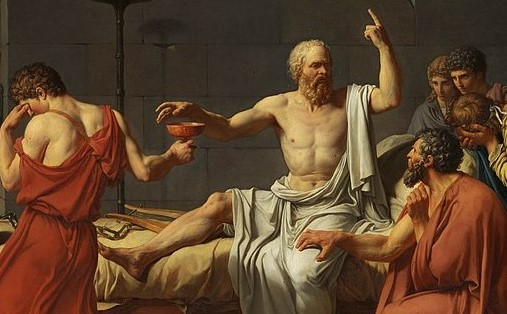
\includegraphics[scale=0.45]{figures/the-death-of-socrates.jpg}
			\vspace*{0.1in}
  		\end{figure}  	
  	\end{itemize}	
  \end{block}
}


%%%%%%%%%%%%%%%%%%%%%%%%%%%%%%%%%%%%%%%%%%%%%%%%%%%%%%%%%%%%%

\frame{
  \frametitle{Logical Consequence}  
  \begin{block}{Logical Consequence}
  	\begin{itemize}
  		\item Every model of the axioms is a model of the conjecture.
  		\item A set of axioms has a \textit{model} if there is an 
  			\textit{interpretation} (assignment of boolean values) to the 
  			axioms such that the conjunction of the axioms evaluate to 
  			\textit{True}.
  		\item If we list all interpretations of $N$ formulae on a truth table, 
  			we get $2^{N}$ rows. This search space grows exponentially.
  		\item The faster way is to show that the union of the axioms and 
  			the negation of the conjecture is \textit{unsatisfiable}. 
  			$Ax \cup \neg C = \emptyset$
  		\item In other words, if no model of the axioms is a model of the
  			negated conjecture, then all models of the axioms are 
  			models of the conjecture.
  	\end{itemize}
  \end{block}
}

%%%%%%%%%%%%%%%%%%%%%%%%%%%%%%%%%%%%%%%%%%%%%%%%%%%%%%%%%%%%%

\frame{
  \frametitle{Problem Statement}  
  \begin{block}{Problem Statement}
  	\begin{itemize}
  		\item A \textit{large-theory} problem consists of a conjecture to be 
  			proven, and a large number of axioms to be considered.
  		\item However, the solution set(s) usually consist of a few axioms.
  		\item How do we select the necessary axioms? This is known as the 
  			problem of \textit{premise selection}.
  	\end{itemize}
  		
  	\begin{figure}[H]
		\centering
		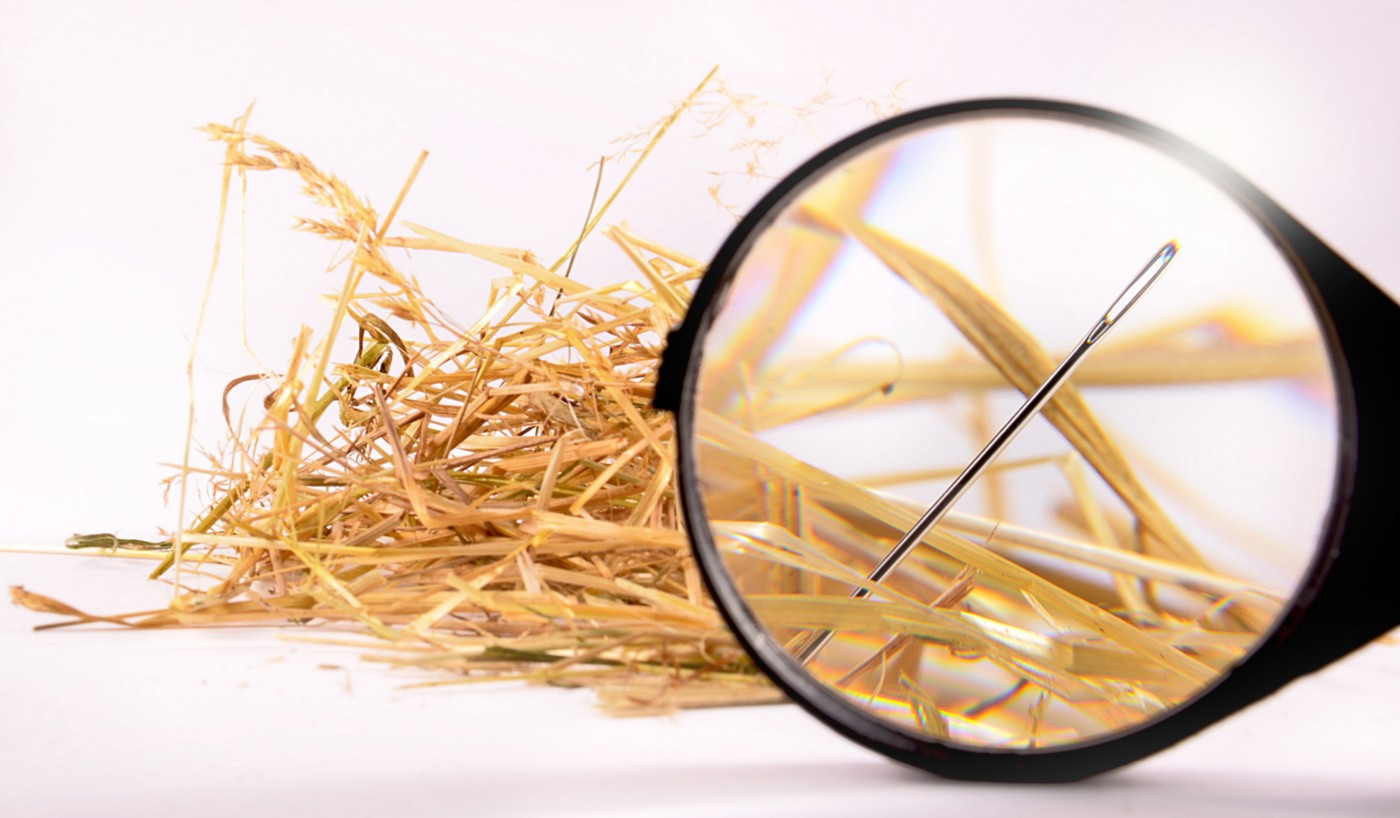
\includegraphics[scale=0.1]{figures/needle-in-haystack.jpeg}
		\vspace*{0.1in}
  	\end{figure}
  \end{block}
}

%%%%%%%%%%%%%%%%%%%%%%%%%%%%%%%%%%%%%%%%%%%%%%%%%%%%%%%%%%%%%

\section{Related Work}
\frame{
  \frametitle{Benchmark Data}  
  \begin{block}{MPTP2078 Dataset}
  	\begin{itemize}
  		\item Benchmark dataset of 2078 problems known as the 
  			Mizar Problems for Theorem Provers (MPTP2078) \cite{AH14}.
  			\begin{itemize}
  	  		\item Encodes problems from the Mizar Mathematical Library (MML) 	
  	  			of formalized mathematics into first-order logic form.
  			\end{itemize}
  		\item There are two versions of each problem:
  		\begin{itemize}
  			\item Bushy = smaller version (3 to 40 axioms, 1 to 15 needed)
  			\item Chainy = larger version (10 to 500 axioms, 2 to 119 needed)	
  		\end{itemize}
  	\item Premise selection performance compared to state-of-the-art 
  		Automated Theorem Provers: 
  		\begin{itemize}
  			\item E \cite{E-Sch13-LPAR}
  			\item Vampire \cite{Vampire-KV13}
  		\end{itemize}	
  	\end{itemize}	
  \end{block}
}

%%%%%%%%%%%%%%%%%%%%%%%%%%%%%%%%%%%%%%%%%%%%%%%%%%%%%%%%%%%%%

\frame{
  \frametitle{Ranking Problem}  
  \begin{block}{Ranking Problem}
  	\begin{itemize}
  		\item Paulson and Blanchette, and Alama et al. formulated premise 
  			selection as a \textit{ranking problem} \cite{PB10, AH14}:
  			\begin{itemize}
  				\item Rank the axioms by how likely they are to prove a 
  					conjecture, based on some kind of user-defined 
  					similarity metric.
  				\item Choose a threshold value.
  				\item Select all axioms whose score is above that threshold.
  			\end{itemize}
  		\item Also a \textit{classification problem}: 
  			\begin{itemize}
  				\item Given a feature matrix consisting of the similarity 
  					values between formulae in a problem, train different 
  					machine learning methods on the data to classify if an 
  					axiom is \textit{likely} or \textit{unlikely} to be in 
  					the proof.
  			\end{itemize}
  	\end{itemize}	
  \end{block}
}

%%%%%%%%%%%%%%%%%%%%%%%%%%%%%%%%%%%%%%%%%%%%%%%%%%%%%%%%%%%%%

\frame{
  \frametitle{Related Work}  
  \begin{block}{Extended Hutchinson Distance}
  	\begin{itemize}
  		\item To construct an adjacency matrix, we require a measure of 
  			similarity or dissimilarity between each pair of nodes in a graph.
  		\item Liu \cite{Liu2017Metric} proposed a dissimilarity metric 
  			between two terms $\Delta_{1}$ and $\Delta_{2}$, that extends 
  			the Hutchinson distance \cite{Hut97}.
  		\item Calculated by finding the Least Generalized Generalization 
  			(\textit{lgg}) between two formulae. A term $\Delta$ is the 
  			\textit{lgg} of $\Delta_{1}$ and $\Delta_{2}$ iff
  			\begin{itemize}
  				\item There are substitutions $\theta_{1}$ and $\theta_{2}$
  					such that $\Delta \theta_{1} = \Delta_{1}$ and 
  					$\Delta \theta_{2} = \Delta_{2}$.
  				\item There exists no term $\Delta'$ and substitutions
  					$\sigma$, $\sigma_{1}$ and $\sigma_{2}$ such that 
  					$\Delta \sigma_{1} = \Delta'$ and 
  					$\Delta \sigma_{2} = \Delta'$.
  			\end{itemize}
  	\end{itemize}	
  \end{block}
}

%%%%%%%%%%%%%%%%%%%%%%%%%%%%%%%%%%%%%%%%%%%%%%%%%%%%%%%%%%%%%

\frame{
  \frametitle{Related Work}  
  \begin{block}{Least Generalized Generalization Example}
  	\begin{itemize}
  	  	\item Note that the substitutions $\theta_{1}$ and $\theta_{2}$ are 
  	  		not limited to a single substitution rule. They can also consist  
  	  		of multiple substitution rules occurring one after the other.
  	\end{itemize}
  	\begin{figure}[H]
  		\centering
		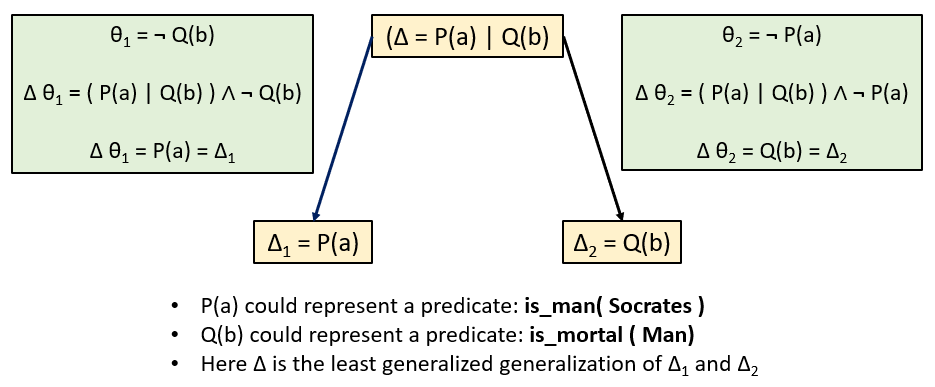
\includegraphics[scale=0.5]{figures/least-generalized-generalization-example.png}
		\vspace*{0.1in}
  	\end{figure}
  \end{block}
}

%%%%%%%%%%%%%%%%%%%%%%%%%%%%%%%%%%%%%%%%%%%%%%%%%%%%%%%%%%%%%

\frame{
  \frametitle{Related Work}  
  \begin{block}{Extended Hutchinson Distance}
  	\begin{itemize}
  		\item If there is no Least Generalized Generalization $\Delta$
  			between two terms $\Delta_{1}$ and $\Delta_{2}$, then their 
  			extended Hutchinson distance is $\infty$. Formally,
  			\textit{dissimilarity}($\Delta_{1}$, $\Delta_{1}$) $= \infty$
  				iff $lgg(\Delta_{1}, \Delta_{2}) = \emptyset$.
  		\item If there exists a Least Generalized Generalization $\Delta$
  			between two terms $\Delta_{1}$ and $\Delta_{2}$, then the 
  			Extended Hutchinson Distance says:
  				\begin{itemize} 
  					\item More total substitutions required (from the 
  					\textit{lgg} to both terms) equates to a higher 
  						dissimilarity score.
  					\item Fewer total substitutions required equates to a 
  						lower dissimilarity score.
  				\end{itemize}
  		\item Note: this is an over-simplication of the actual metric.
  		\item As expected, for any term $\Delta_{1}$,
			\textit{dissimilarity($\Delta_{1}$, $\Delta_{1})$} = 0
  	\end{itemize}	
  \end{block}
}

%%%%%%%%%%%%%%%%%%%%%%%%%%%%%%%%%%%%%%%%%%%%%%%%%%%%%%%%%%%%%

\frame{
  \frametitle{Graph Matrices}  
  \begin{block}{Graph Laplacian Matrix}
  	\begin{itemize}
  		\item Von Luxburg \cite{vonLuxburg2007} describes this technique to 
  			cluster vertices in an undirected graph according to some 
  			user-defined similarity metric.
  		\item Adjacency matrix $A$ consists of edge weights between pairs 
  			of vertices that represent their similarity.
  		\item Degree matrix $D$ is a diagonal matrix where the $i^{th}$ 
  			element is the sum of the elements of the $i^{th}$ column of $A$.
  		\item Un-normalized Graph Laplacian matrix.
		\begin{itemize}
			\item $L = D\ –\ A$
		\end{itemize}
		\item Normalized Graph Laplacian matrix contains \textit{features}
			of the graph
		\begin{itemize}
			\item $L_{norm} = I\ –\ (D^{-1/2}\ L\ D^{-1/2})$
		\end{itemize}
  	\end{itemize}	
  \end{block}
}

%%%%%%%%%%%%%%%%%%%%%%%%%%%%%%%%%%%%%%%%%%%%%%%%%%%%%%%%%%%%%

\frame{
  \frametitle{Example Graph}  
  \begin{block}{Calculate Normalized Laplacian Matrix}
  	\begin{itemize}
  		\item Adjacency, Degree, and Un-normalized Graph Laplacian
  		\[ 
  		A = \begin{bmatrix}
		0 & 3 & 0 \\
		3 & 0 & 1 \\
		0 & 1 & 0
		\end{bmatrix} 
		\quad
		D = \begin{bmatrix}
		3 & 0 & 0 \\
		0 & 4 & 0 \\
		0 & 0 & 1
		\end{bmatrix}
		\quad
		L = \begin{bmatrix}
		0 & 3 & 0 \\
		3 & 0 & 1 \\
		0 & 1 & 0
		\end{bmatrix}
		\]
		\item Normalized Graph Laplacian
		\[ 
  		L_{norm} = \begin{bmatrix}
		1 & 0 & 0 \\
		0 & 1 & 0 \\
		0 & 0 & 1
		\end{bmatrix} -
		\begin{bmatrix}
		\dfrac{1}{\sqrt{3}} & 0 & 0 \\
		0 & 1/2 & 0 \\
		0 & 0 & 1
		\end{bmatrix} 
		\begin{bmatrix}
		0 & 3 & 0 \\
		3 & 0 & 1 \\
		0 & 1 & 0
		\end{bmatrix}
		\begin{bmatrix}
		\dfrac{1}{\sqrt{3}} & 0 & 0 \\
		0 & 1/2 & 0 \\
		0 & 0 & 1
		\end{bmatrix} 
		\]
  	\end{itemize}	
  \end{block}
}

%%%%%%%%%%%%%%%%%%%%%%%%%%%%%%%%%%%%%%%%%%%%%%%%%%%%%%%%%%%%%
\section{Methodology}

\frame{
  \frametitle{Evaluation Metrics}  
  \begin{block}{Definitions}
	\begin{itemize}
		\item The \emph{N}umber of \emph{Ax}ioms in a \emph{P}roblem: 		
			\emph{NAxP}.
		\item The \emph{N}umber of axioms \emph{Sel}ected: \emph{NSel}.
		\item The \emph{N}umber of axioms \emph{N}eeded \emph{f}or a 
			\emph{P}roof, i.e., the number of axioms in an adequate set
			\emph{NNfP}.
	\end{itemize}
  \end{block}
}

%%%%%%%%%%%%%%%%%%%%%%%%%%%%%%%%%%%%%%%%%%%%%%%%%%%%%%%%%%%%%

\frame{
  \frametitle{Evaluation Metrics}  
  \begin{block}{Precision and Selectivity Metrics}
  	\begin{itemize}
  	  	\item \textbf{Precision} \\
			If the axiom selection technique selects an adequate set of 
				axioms (i.e. set that is known to lead to a proof), then 
				\textbf{precision} is the minimum \emph{NNfP}$/$\emph{NSel} 
				over the known adequate sets of axioms. \\
				
			Otherwise, if it selects an inadequate set, then 
				\textbf{precision} is $0$. \\
				
			Larger values are better because it means that fewer 
				unnecessary axioms were selected.
		
		\item \textbf{Selectivity}: \emph{NSel}$\ /$\ \emph{NAxP} \\
		  	The fraction of axioms selected from the problem, regardless of
		  	whether an adequate set was selected or not. Smaller values are 
		  	better.
  	\end{itemize}
  \end{block}
}

%%%%%%%%%%%%%%%%%%%%%%%%%%%%%%%%%%%%%%%%%%%%%%%%%%%%%%%%%%%%%

\frame{
  \frametitle{Evaluation Metrics}  
  \begin{block}{Average and Adequacy Metrics}
  	\begin{itemize}
  		\item \textbf{Average precision/selectivity/precision} \\
  			For a set of problems, the average value of the metric over the
  			problems.
		\item \textbf{Adequacy} \\
		  	For a set of problems, the fraction of problems for which the 
		  	axiom selection technique selects an adequate set of axioms.
		  	Larger values are better.
  		\item \textbf{Adequate precision/selectivity/precision} \\
			For a set of problems, the average over the problems for which the 
			axiom selection technique selects an adequate set of axioms.
  	\end{itemize}
  \end{block}
}

%%%%%%%%%%%%%%%%%%%%%%%%%%%%%%%%%%%%%%%%%%%%%%%%%%%%%%%%%%%%%

\frame{
  \frametitle{Methodology}  
  \begin{block}{Graph Representation}
  	\begin{itemize}
  		\item Use Extended Hutchinson distance to get dissimilarity values 
  			of all pairs of vertices in a problem.
  		\item Let $\Phi_1$ and $\Phi_1$ represent two formulae with 
  		dissimilarity of $dsim(\phi_i,\phi_j)$. We convert dissimilarity 
  		values into similarity values using the following formula:
  			\begin{align}
  				maxdsim(\mathcal{F}) &= max_{\phi_i,\phi_j \in \mathcal{F}} (dsim(\phi_i,\phi_j) \neq \infty) \\
  				sim(\Phi_1,\Phi_2,\mathcal{F}) &= \textrm{max}(0, maxdsim(\mathcal{F}) - dsim(\Phi_1,\Phi_2))
  			\end{align}
  		\item The logic problem becomes a fully-connected and undirected graph
  		\begin{itemize}
  			\item Vertices $V$ = $\{$Axioms $\cup$ Conjecture$\}$
  			\item Edges $E$ = weighted by similarity between vertices  		
  		\end{itemize}
  	\end{itemize}	
  \end{block}
}

%%%%%%%%%%%%%%%%%%%%%%%%%%%%%%%%%%%%%%%%%%%%%%%%%%%%%%%%%%%%%

\frame{
  \frametitle{Spectral Clustering Algorithm}  
  \begin{block}{Spectral Clustering \cite{vonLuxburg2007}}
  		\begin{enumerate}
    		\item Construct a weight matrix W (i.e. adjacency matrix A) 
    		containing similarity values of the edges of the graph.
  			\item Compute the normalized Laplacian matrix $L_{norm}$ from $W$.
			\item Compute the first $k$ eigenvectors $v_{1}, ..., v_{k}$ of 
				$L_{norm}$ and construct a feature matrix $U$ from those 
				eigenvectors.
			\item For $i = 1, ..., n$, let $p_{i}$ be the feature vector for 
				the $i^{th}$ vertex, corresponding to the $i^{th}$ row of $U$.
			\item Cluster the vertices based on their feature vectors into 
				$k$ clusters: $C_{1}, C_{2}, ..., C_{k}$. Denote the cluster 
				containing the conjecture as $C_{C}$.
  		\end{enumerate}		
  \end{block}
}

%%%%%%%%%%%%%%%%%%%%%%%%%%%%%%%%%%%%%%%%%%%%%%%%%%%%%%%%%%%%%

\frame{
  \frametitle{K-Means Clustering}  
  \begin{block}{Problems with K-Means Clustering}
  	\begin{itemize}
  		\item First, each run of k-means chooses a different set of initial 
  			centroids for the $k$ clusters. This results in a different 
  			clustering each time.
  	  	\item We need deterministic way of initializing the centroids
  	  		of the $k$ clusters.
		\item Second, we need to figure out the optimal value for the 
			parameter $k$, the number of clusters.
  	\end{itemize}
  \end{block}
}

%%%%%%%%%%%%%%%%%%%%%%%%%%%%%%%%%%%%%%%%%%%%%%%%%%%%%%%%%%%%%

\frame{
  \frametitle{K-Means Clustering}  
  \begin{block}{Solution to Initial Centroids Problem}
  	\begin{itemize}
    	\item The \textit{degree centrality} of a vertex $v$ is the sum of the 
    		weights of all the edges connected to $v$. 
    	\item Rank the vertices in descending order by their degree centrality.
    	\item Select the top $(k - 1)$ most central vertices and the 
    		conjecture. Use their feature vectors from the matrix $U$ as the
    		initial centroids for the $k$ clusters.
  	\end{itemize}
  \end{block}
}

%%%%%%%%%%%%%%%%%%%%%%%%%%%%%%%%%%%%%%%%%%%%%%%%%%%%%%%%%%%%%

\frame{
  \frametitle{K-Means Clustering}  
  \begin{block}{Solution to Optimal Number of Clusters Problem}
  	\begin{itemize}
  		\item Let \emph{NAxP} denote the number of axioms in a logic problem.
    	\item Brute force: try all values of $k$ from $2$ to \emph{NAxP}. 
    	\item For each problem, record the $k$ number of clusters that gives
    		us the best \textbf{precision} value. Call this the optimal $k$.
    	\item Recall that \textbf{precision} is \textit{the minimum number of 
    		axioms needed for a proof} divided by \textit{the number of axioms 
    		selected by the axiom selection technique}.
  	\end{itemize}
  \end{block}
}

%%%%%%%%%%%%%%%%%%%%%%%%%%%%%%%%%%%%%%%%%%%%%%%%%%%%%%%%%%%%%

\frame{
  \frametitle{Predict Optimal Number of Clusters}  
  \begin{block}{Median Regression}
  	\begin{itemize}
    	\item Use median regression to create a regression line where the 
    		y-axis is the optimal $k$ and the x-axis is the number of axioms
    		in the problem.
    	\item For each problem, use the regression line to predict the optimal 
    		$k$ based on the number of axioms in the problem. Denote the 
    		predicted value as $k_{pred}$.
    	\item For each problem, run spectral clustering using $k_{pred}$ and 
    		record the precision, selectivity, and adequacy.
  	\end{itemize}
  \end{block}
}

%%%%%%%%%%%%%%%%%%%%%%%%%%%%%%%%%%%%%%%%%%%%%%%%%%%%%%%%%%%%%
\section{Results}

\frame{
  \frametitle{Results}  
  \begin{block}{Predicted Number of Clusters for Bushy}
  	\begin{figure}[H]
  		\vspace*{0.1in}
		\centering
		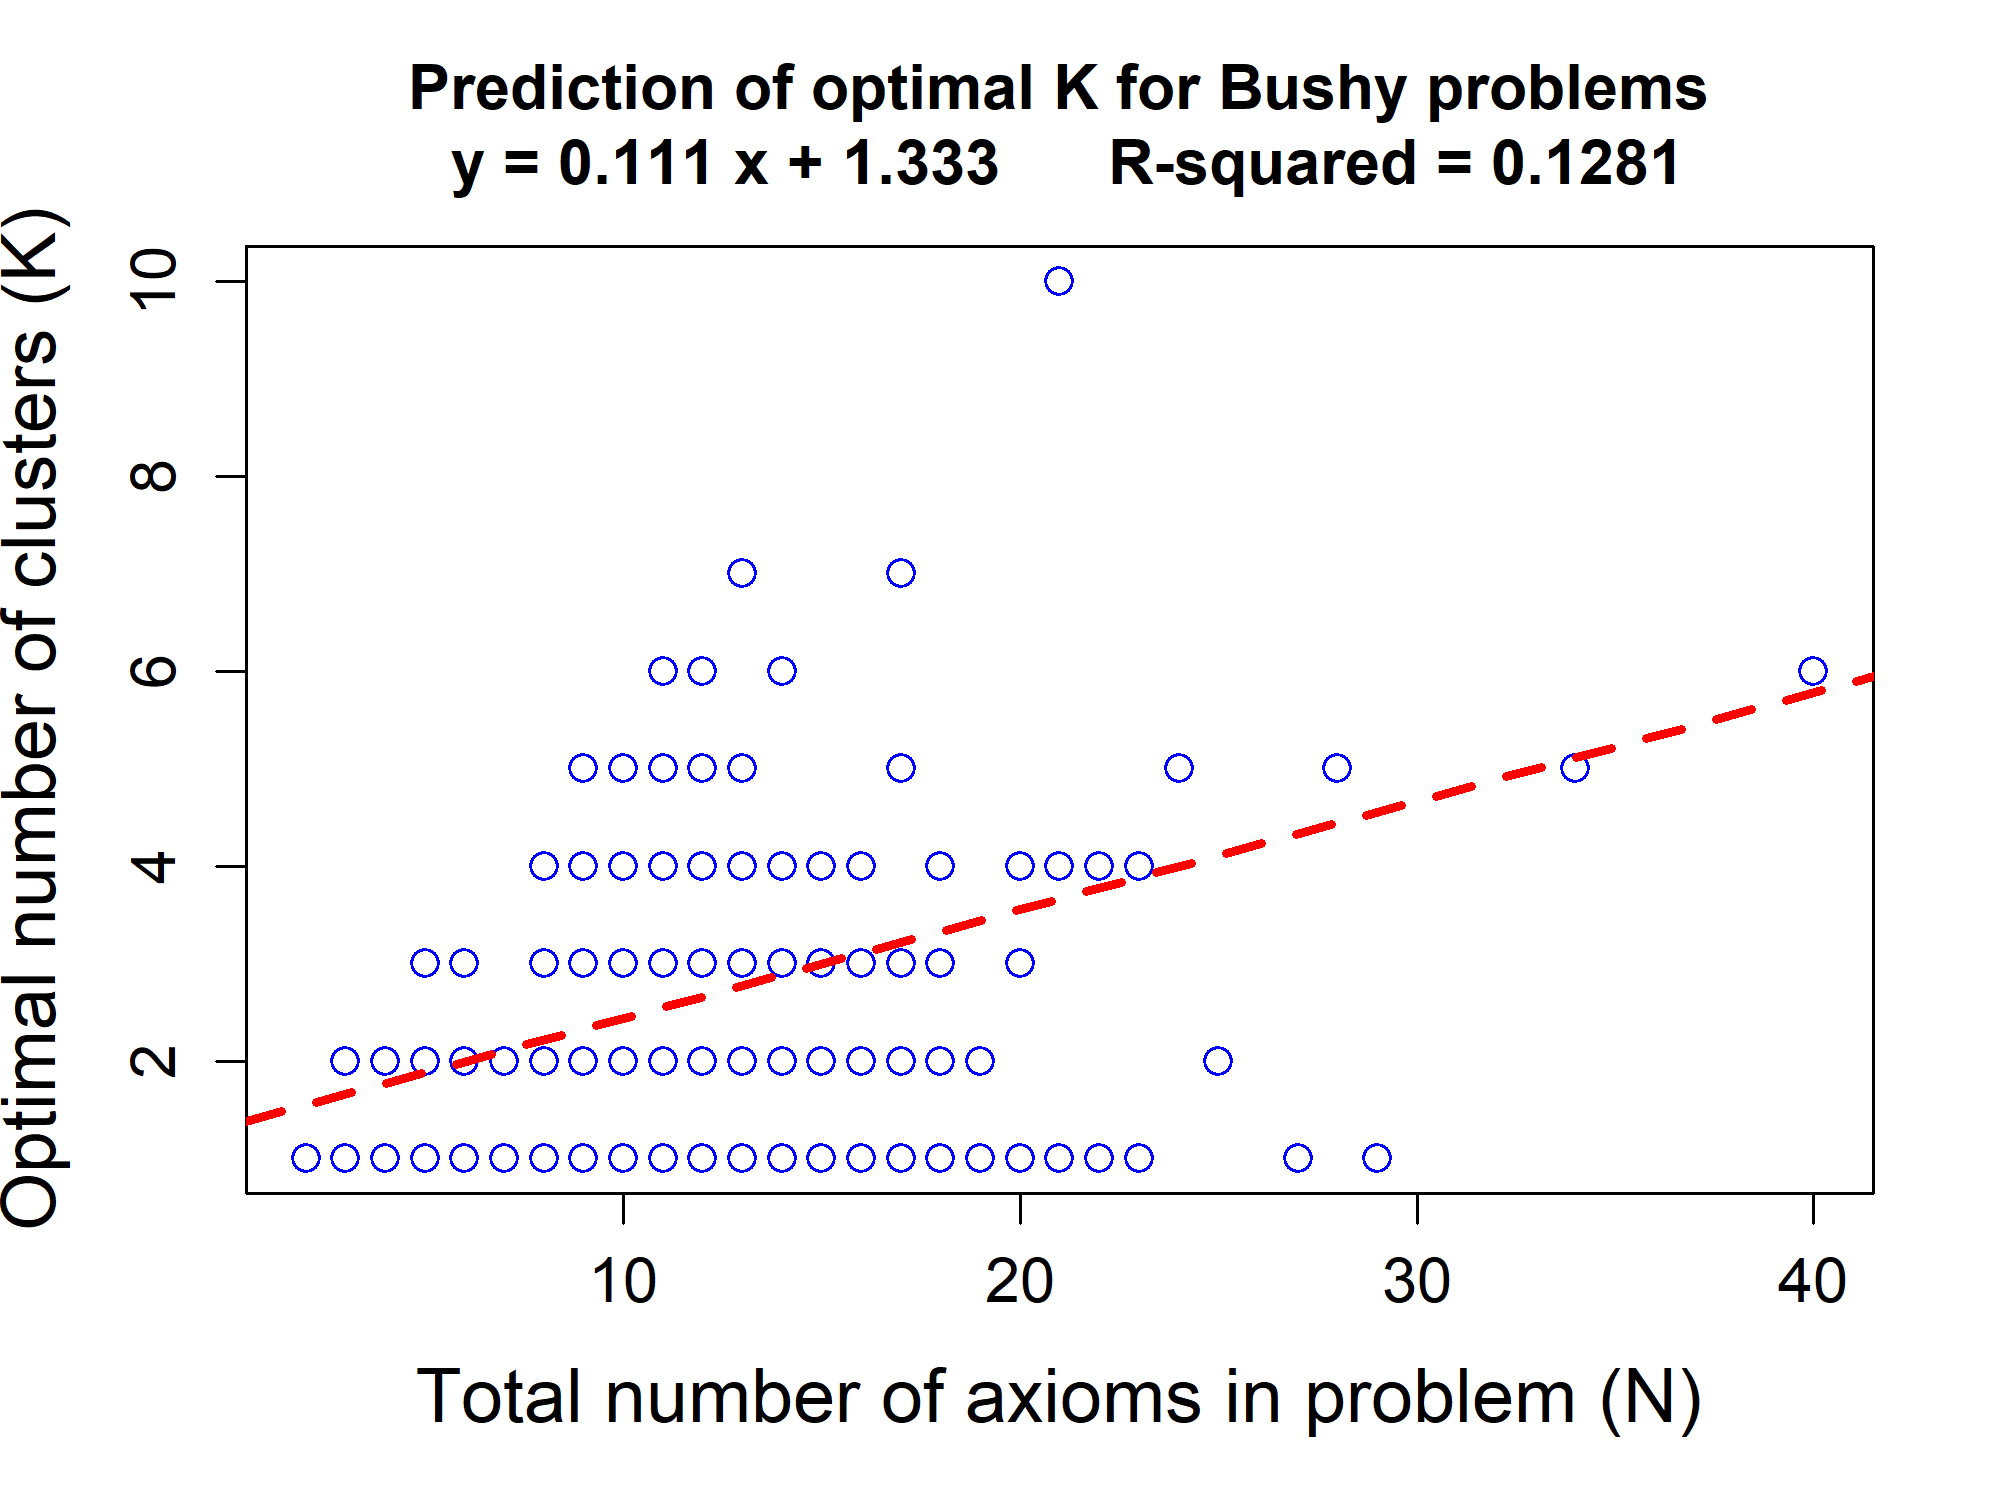
\includegraphics[scale=0.4]{figures/median-regression-optimal-k-bushy.png}
		\vspace*{0.1in}
  	\end{figure}
  \end{block}
}

%%%%%%%%%%%%%%%%%%%%%%%%%%%%%%%%%%%%%%%%%%%%%%%%%%%%%%%%%%%%%

\frame{
  \frametitle{Results}  
  \begin{block}{Predicted Number of Clusters for Chainy}
  	\begin{figure}[H]
  		\vspace*{0.1in}
		\centering
		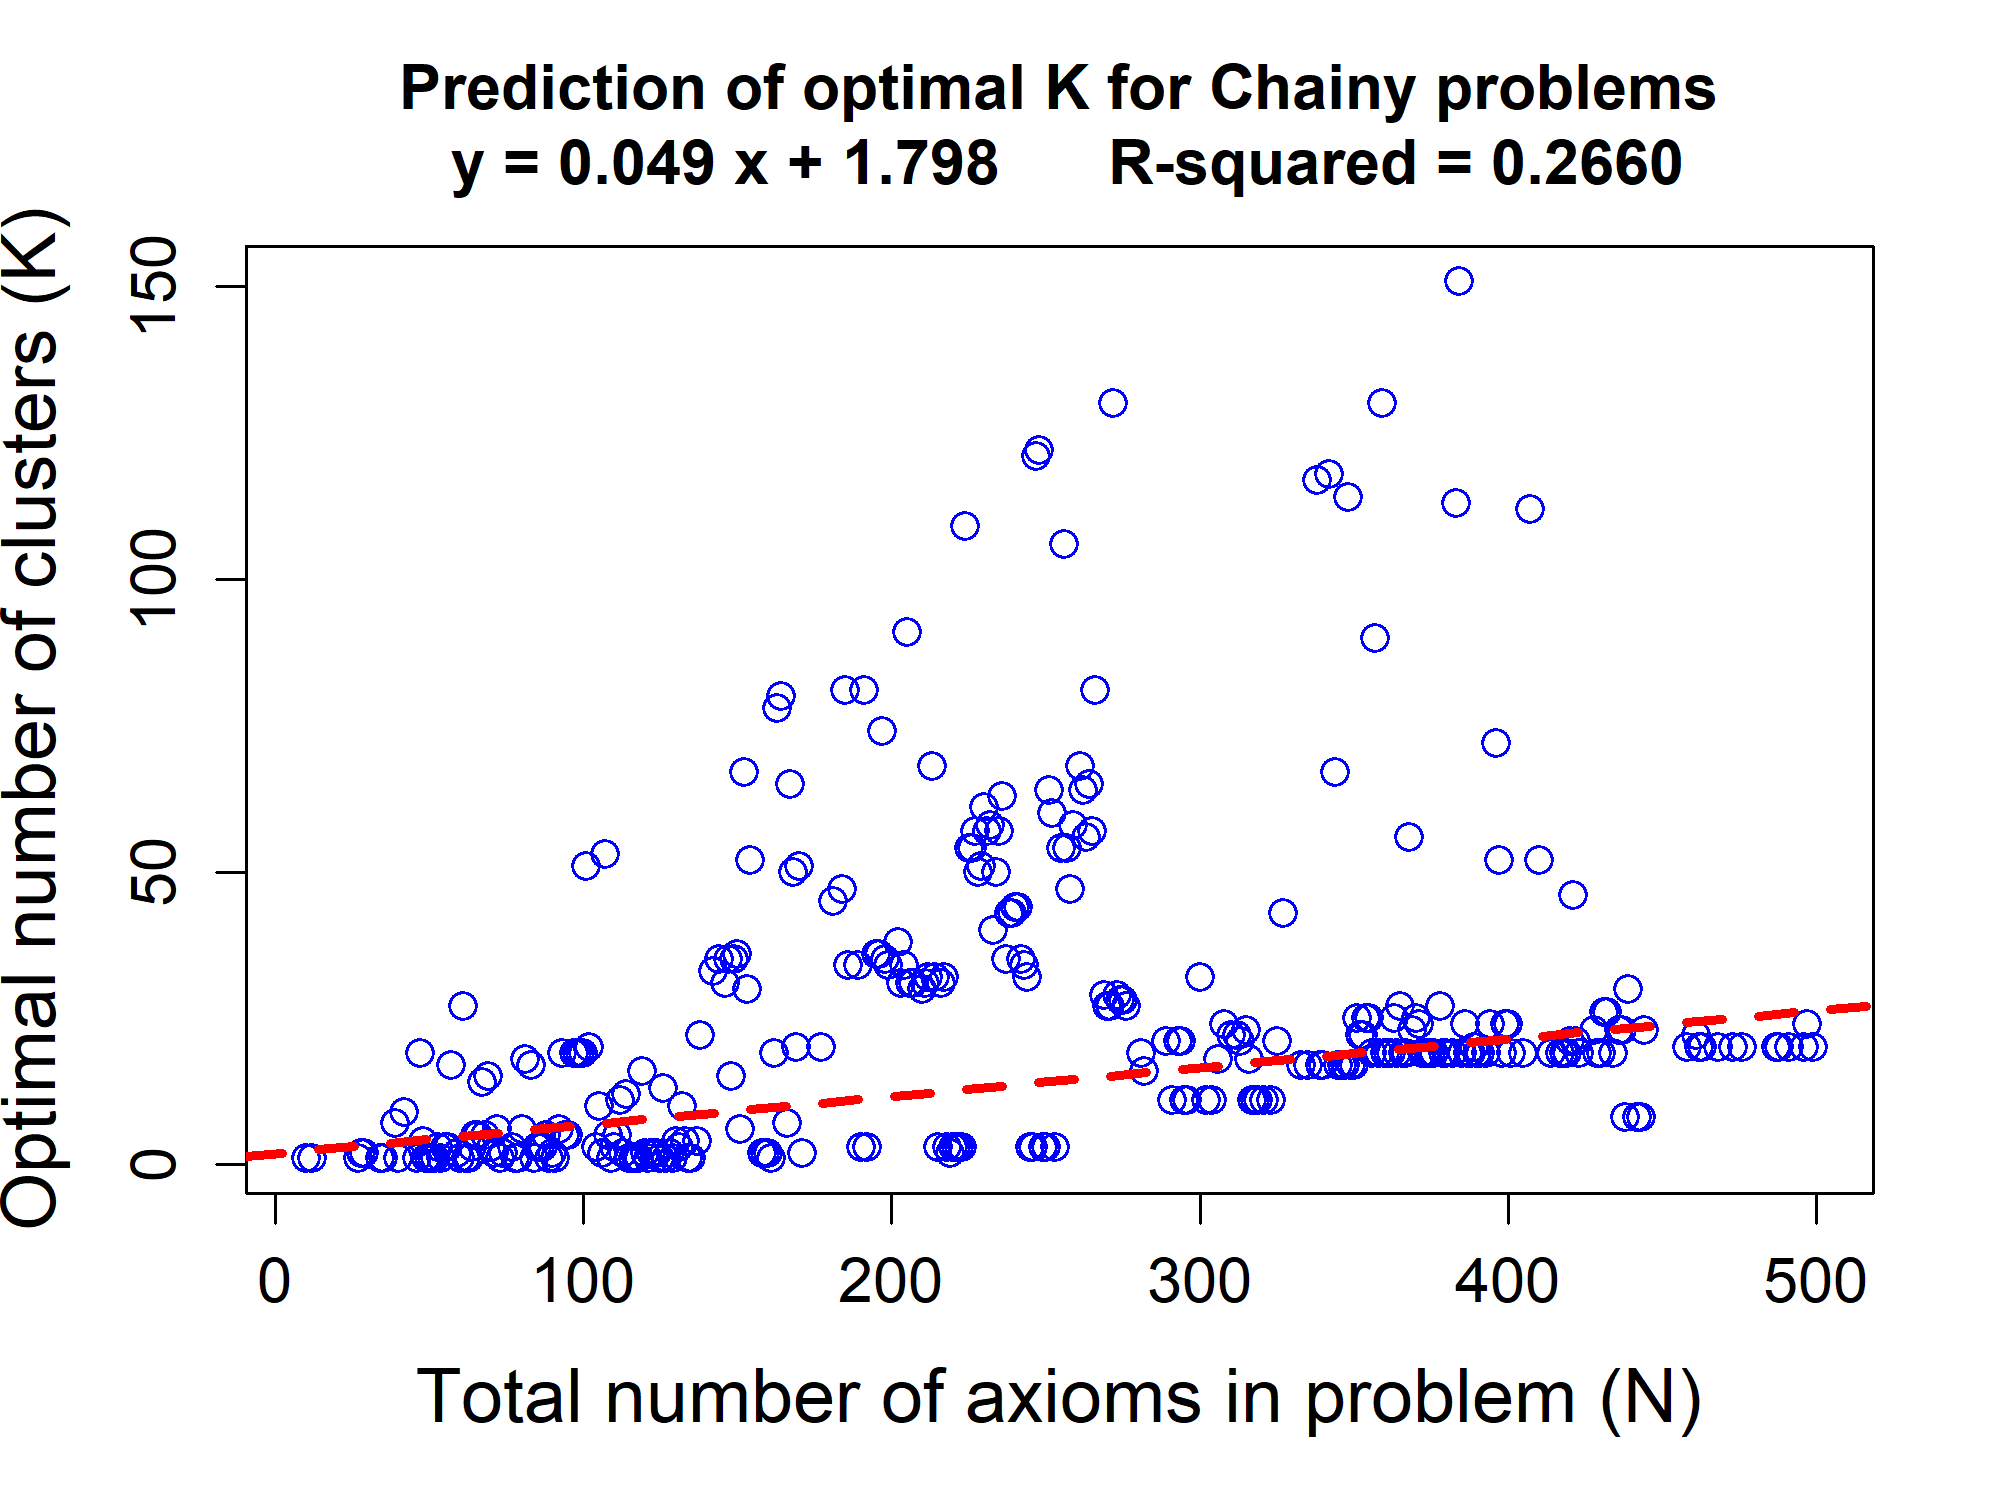
\includegraphics[scale=0.4]{figures/median-regression-optimal-k-chainy.png}
		\vspace*{0.1in}
  	\end{figure}
  \end{block}
}

%%%%%%%%%%%%%%%%%%%%%%%%%%%%%%%%%%%%%%%%%%%%%%%%%%%%%%%%%%%%%

\frame{
  \frametitle{Results}  
  \begin{block}{Evaluation on 325 Bushy and Chainy Problems}
    \begin{figure}[H]
  		\vspace*{0.1in}
		\centering
		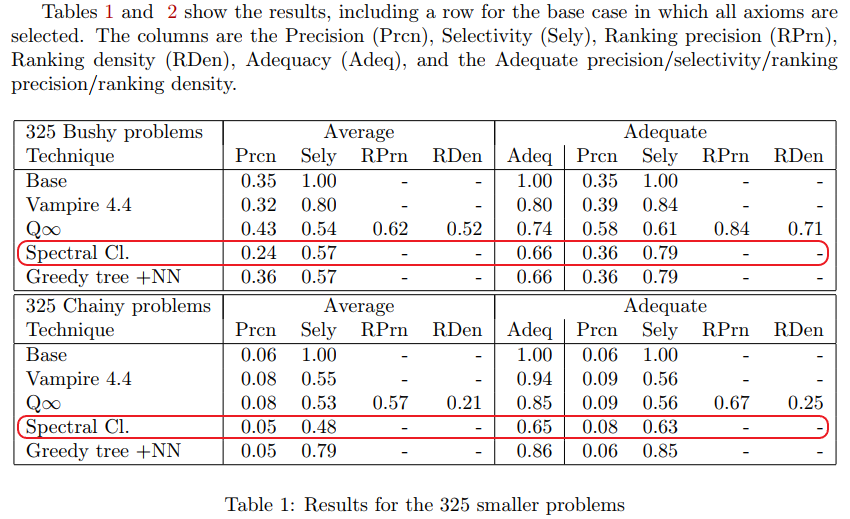
\includegraphics[scale=0.38]{figures/result-325-problems.png}
		\vspace*{0.1in}
  	\end{figure}
  \end{block}
}

%%%%%%%%%%%%%%%%%%%%%%%%%%%%%%%%%%%%%%%%%%%%%%%%%%%%%%%%%%%%%

\frame{
  \frametitle{Results}  
  \begin{block}{Evaluation on 325 Bushy and Chainy Problems}
    \begin{itemize}
    	\item Spectral Clustering is more selective than E and Vampire. 
    		However, this lead it to perform the worst in terms of selecting
    		an adequate set of axioms, for both Bushy and Chainy problems.
    	\item Spectral Clustering performs equally as well as E and Vampire
    		in terms of precision for the problems on which it selects an
    		adequate set of axioms, for both Bushy and Chainy problems.
    		This means when Spectral Clustering does select an adequate set,
    		it is good at removing unnecessary axioms.
    	\item $Q_{\infty}$ is Qinghua's method of removing all axioms with
    		infinite dissimilarity to the conjecture. It's a simple method 
    	 	that performs very well, beating Vampire in terms of selectivity
    	 	and on par with Vampire in terms of precision.
    \end{itemize}
  \end{block}
}


%%%%%%%%%%%%%%%%%%%%%%%%%%%%%%%%%%%%%%%%%%%%%%%%%%%%%%%%%%%%%
\section{Conclusion}

\frame{
  \frametitle{Conclusion}  
  \begin{block}{Conclusion}
  	\begin{itemize}
    	\item Ranking and clustering methods for premise selection depend on
    		how well the ranking metric (whether based on dissimilarity or
    		similarity) manages to capture the relationship between the
    		logical formulae. 
    	\item If the ranking metric is not good, then it affects everything
    		downstream. Therefore, the next step is to validate different
    		ranking metrics, including the Extended Hutchinson Distance.
    	\item Sometimes the simple method (e.g. $Q_{\infty}$) performs better
    		than the complex method (e.g. Spectral Clustering).
  	\end{itemize}
  \end{block}
}

%%%%%%%%%%%%%%%%%%%%%%%%%%%%%%%%%%%%%%%%%%%%%%%%%%%%%%%%%%%%%

\frame{
  \frametitle{Acknowledgements}  
  \begin{block}{Acknowledgements}
  	\begin{itemize}
  	    \item Our paper \textit{Evaluation of Axiom Selection Techniques}
    		was submitted to PAAR 2020 (Workshop on Practical Aspects of 
    		Automated Reasoning) in May 2020.
    	\item Thanks to co-authors: Qinghua Liu, Zihao Wang, 
    		Professor Geoff Sutcliffe.
    	\item Thanks to Jack McKeown for suggesting the use of quantile 
    		regression. At the $50^{th}$ quantile, this becomes median 
    		regression.
    	\item Thanks to Professor Kamal Premaratne for suggesting the use of 
    		spectral clustering.
  	\end{itemize}
  \end{block}
}

%%%%%%%%%%%%%%%%%%%%%%%%%%%%%%%%%%%%%%%%%%%%%%%%%%%%%%%%%%%%%

\bibliographystyle{alpha}
\bibliography{references}

%%%%%%%%%%%%%%%%%%%%%%%%%%%%%%%%%%%%%%%%%%%%%%%%%%%%%%%%%%%%%

\end{document}
